\documentclass[border=1mm]{standalone}

\usepackage[dvipsnames]{xcolor}
\usepackage{tikz}

\usepackage[dvipsnames]{xcolor}
\usepackage{hyperref}

\colorlet{myblue}{RoyalBlue}
\colorlet{myred}{WildStrawberry}
\colorlet{myorange}{Melon}
\colorlet{mygreen}{OliveGreen}
\colorlet{myviolet}{RoyalPurple}
\colorlet{myyellow}{Goldenrod}
\hypersetup{urlbordercolor=Green, linkbordercolor=Blue}

\begin{document}
	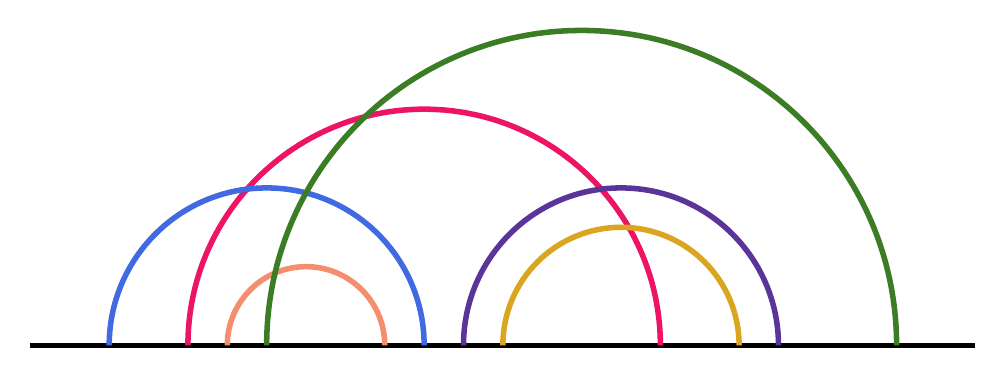
\begin{tikzpicture}[th/.style = {line width = 2pt}]
		\draw[th] (0,0) -- (12,0);
		\draw[color=myred, th] (2,0) arc (180:0:3);
		\draw[color=myblue, th] (1,0) arc (180:0:2);
		\draw[color=myorange, th] (2.5,0) arc (180:0:1);
		\draw[color=myyellow, th] (6,0) arc (180:0:1.5);
		\draw[color=mygreen, th] (3,0) arc (180:0:4);
		\draw[color=myviolet, th] (5.5,0) arc (180:0:2);
	\end{tikzpicture}
\end{document}